% !TEX program = xelatex
% =============================================================================
% 대한수의사회(KVMA) 정기학술대회 발표초록 초고
% - 구조: 국·영문 제목 / 저자·소속 / 목적·재료및방법·결과·고찰 / 핵심어
% - 컴파일(권장): XeLaTeX
%     xelatex kvma_conference_draft.tex
% - Overleaf: Compiler = XeLaTeX, TeX Live 권장
% - 실제 투고 전: 해당 연도 공고의 글자수·여백·글꼴·첨부양식을 반드시 대조할 것
% - 저자·소속·연락처는 예시 자리표시자임
% =============================================================================
\documentclass[10pt,a4paper]{article}

\usepackage{kotex}
\usepackage[margin=20mm]{geometry}
\usepackage{setspace}
\usepackage{booktabs}
\usepackage{array}
\usepackage{graphicx}
\usepackage{caption}
\usepackage{hyperref}
\usepackage{enumitem}
\usepackage{xcolor}

% paper/ 에서 컴파일할 때와 프로젝트 루트에서 컴파일할 때 모두 대응
\graphicspath{{../results/}{results/}}
\captionsetup{font=small,labelfont=bf,skip=0.4em}

\setstretch{1.35}
\setlength{\parindent}{0pt}
\setlength{\parskip}{0.45em}
\setlist[itemize]{leftmargin=1.4em,itemsep=0.15em,topsep=0.25em}
\hypersetup{colorlinks=true,linkcolor=black,urlcolor=blue!50!black}

\newcommand{\presenter}[1]{\underline{#1}} % 발표자 밑줄
\newcommand{\meta}[1]{\noindent{\small #1}\par}

\begin{document}

% ----- 투고 메타 (공고 항목에 맞춰 수정) -----
\begin{center}
{\footnotesize
대한수의사회 정기학술대회 발표초록 초고}\\[0.2em]
{\footnotesize
발표형태: 구두 / 포스터\quad|\quad
분과: 돼지$\cdot$예방수의학\quad|\quad
원저 / 단보}
\end{center}

\vspace{0.4em}

% ----- 제목 -----
\begin{center}
{\large\bfseries
카메라 기반 일별 활력도 변화와\\
향후 3일 이내 돼지 질병 확인 위험의 연관성 평가}\\[0.55em]
{\normalsize\itshape
Association between camera-based daily vitality changes\\
and risk of veterinarian-confirmed disease within 3 days in pigs}\\[0.9em]
{\normalsize
\presenter{홍길동}$^{1}$\textsuperscript{*},\; 김철수$^{1}$}\\[0.35em]
{\small $^{1}$○○대학교 수의과대학}\\[0.25em]
{\small \textsuperscript{*}교신저자: hong@example.ac.kr}
\end{center}

\vspace{0.3em}
\begin{center}\rule{0.92\textwidth}{0.4pt}\end{center}

% ----- 구조화 초록 본문 -----
\section*{목\;적}
돼지는 질병 초기에 이동량, 섭식$\cdot$음수, 자세 및 사회적 접촉이 달라질 수 있으나, 순회 관찰만으로 개체-일 단위의 미세 변화를 연속적으로 확인하기는 어렵다. 본 연구는 영상$\cdot$환경센서에서 산출한 일별 활력도와 최근 3일 변화량이, 향후 3일 이내 수의사 확인 질병 위험을 어느 정도 구분하는지 평가하였다. 출력은 진단이 아니라 관찰 우선순위를 정하기 위한 조기경보 위험도로 해석한다.

\section*{재료 및 방법}
교육용 \textbf{합성} 관찰자료를 사용하였다(8돈방, 돼지 120두, 관찰 42일). 원자료는 개체 메타데이터 120행, 일별 관찰 5,045행, 수의사 확인 질병 이벤트 36건이었다. 품질관리(완전 중복 제거, \texttt{valid}=False 제외, 카메라 커버리지 70\% 미만 및 범위 오류 제외) 후 라벨$\cdot$과거 변화량을 결합한 분석용 자료 4,269 개체-일(양성 105, 양성률 2.46\%)을 분석하였다.

측정단위는 개체-일(pig-day)이다. 결과변수 \texttt{disease\_next\_3d}는 관찰일 다음 날부터 3일 이내 임상발현일 존재 여부로 정의하였다. 처치일$\cdot$회복일$\cdot$확인일은 예측변수로 사용하지 않았다. 과거 변화량은 관찰일 이전 최대 3일 중앙값 대비 차이(\texttt{vitality\_delta\_3d}, \texttt{activity\_delta\_pct\_3d}) 및 이전 3일 기침 합(\texttt{cough\_events\_prior\_3d})으로 산출하였다.

비교 모형은 다음과 같다.
\begin{itemize}
  \item \textbf{M0}(기초): 일령, 체중, 온도, 습도, 돈방
  \item \textbf{M1}(당일 활력): M0 + 당일 행동$\cdot$활력도$\cdot$카메라 커버리지
  \item \textbf{M2}(변화): M1 + \texttt{vitality\_delta\_3d}, \texttt{activity\_delta\_pct\_3d}, \texttt{cough\_events\_prior\_3d}
\end{itemize}
분류기는 class-weight 균형 로지스틱 회귀이며, 범주형은 one-hot, 연속형은 중앙값 대치 후 표준화하였다. 자료는 연구일 기준 시간순으로 분할하였다(train 0--25일, validation 26--33일, test 34--41일; 각각 $n$=2,860 / 743 / 666). 동일 개체의 인접일을 임의 행 분할하지 않았다. 임계값은 validation에서 민감도 $\geq 0.80$을 만족하는 후보 중 정밀도 최대로 선택하고, test는 최종 1회만 평가하였다. 주지표는 AUPRC이며, 보조지표로 AUROC, 민감도, 특이도, 양성예측도(PPV), 돼지 100두$\cdot$일당 경보 수를 보고하였다.

\section*{결\;과}
양성(\texttt{disease\_next\_3d}=1) 개체-일의 \texttt{vitality\_delta\_3d} 평균은 $-9.57$로, 음성($-0.12$)보다 낮았다(그림~\ref{fig:eda}). 임상발현 전 7일 평균 궤적에서도 \texttt{vitality\_score}와 \texttt{vitality\_delta\_3d}가 발현 접근에 따라 하락하는 경향을 보였다(그림~\ref{fig:traj}).

\begin{figure}[ht]
\centering
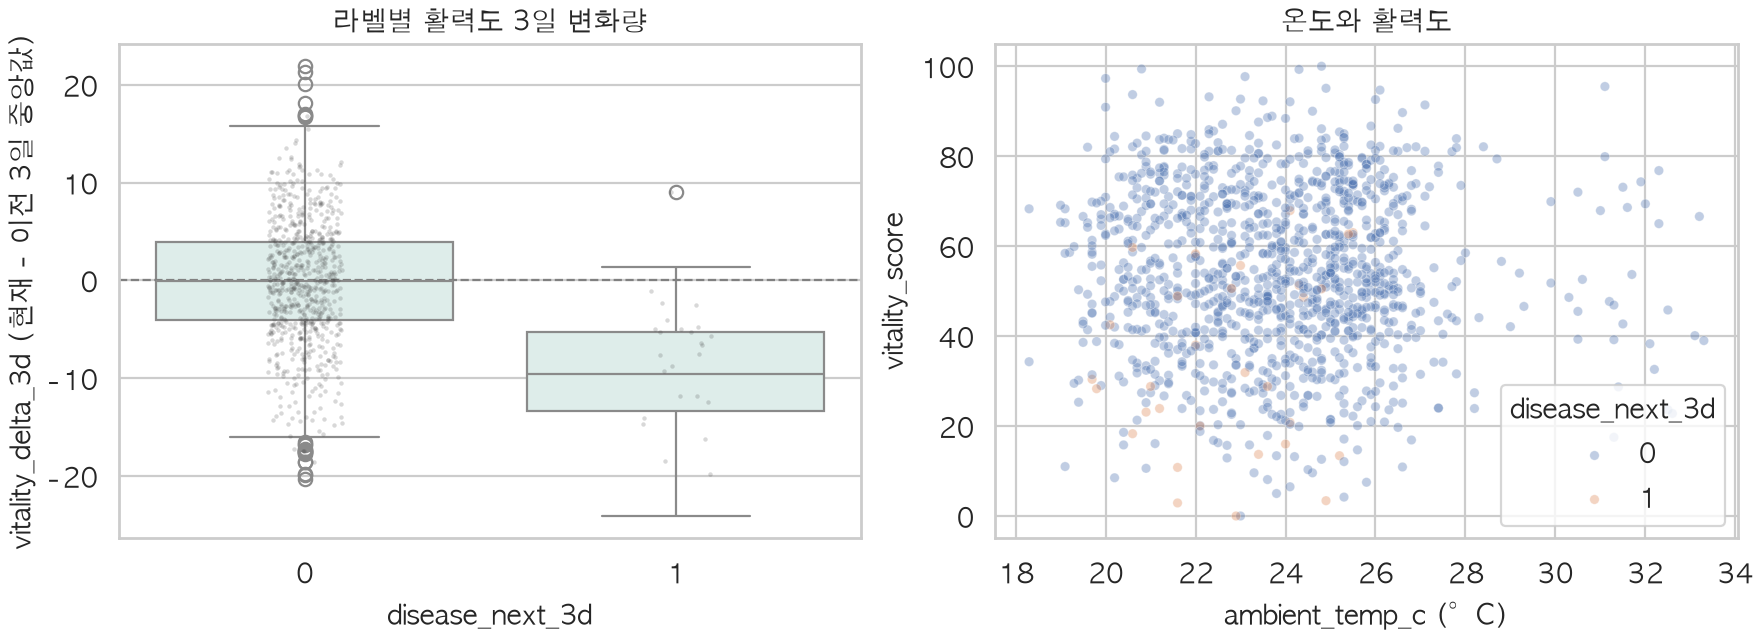
\includegraphics[width=0.92\textwidth]{thesis_eda_vitality.png}
\caption{라벨별 \texttt{vitality\_delta\_3d} 분포(좌)와 온도와 활력도 산점도(우). 양성군에서 최근 3일 기준선 대비 활력도 저하가 뚜렷하다.}
\label{fig:eda}
\end{figure}

\begin{figure}[ht]
\centering
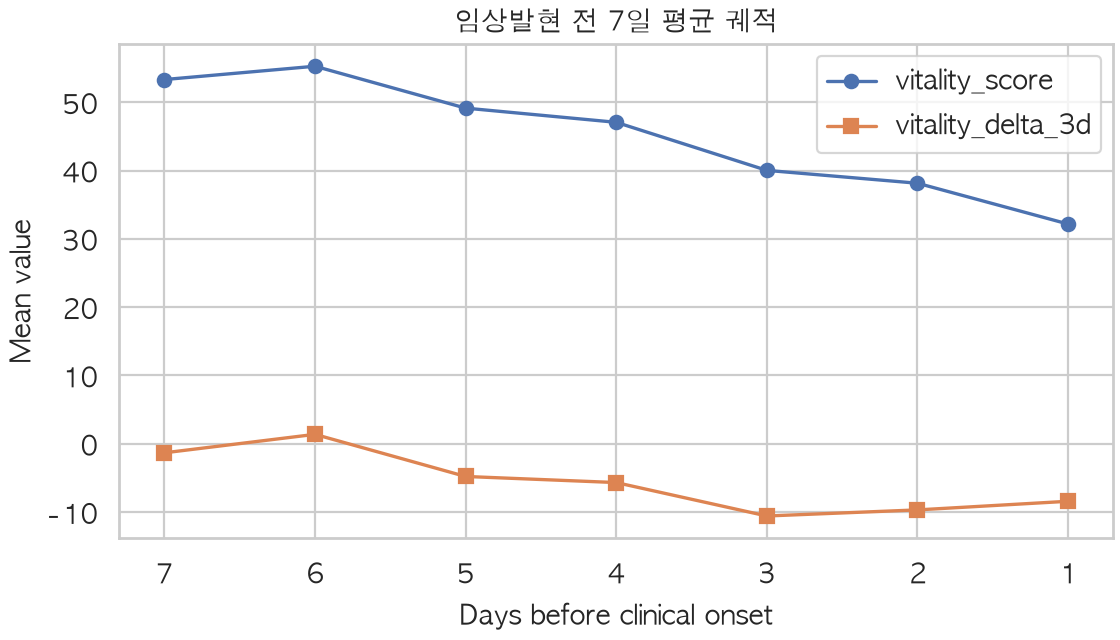
\includegraphics[width=0.72\textwidth]{thesis_onset_trajectory.png}
\caption{임상발현 전 7일간 활력도(\texttt{vitality\_score})와 3일 변화량(\texttt{vitality\_delta\_3d})의 평균 궤적.}
\label{fig:traj}
\end{figure}

검사자료(test; $n$=666, 양성 25, 양성률 3.75\%)에서 모형 성능은 표~\ref{tab:metrics}과 같다. AUPRC는 M0 0.051, M1 0.488, M2 0.759였고, AUROC는 각각 0.574, 0.901, 0.982였다. validation에서 정한 임계값을 test에 적용했을 때 M2의 민감도는 0.68, PPV 0.77, 경보량은 3.3/100 pig-days였다. M0은 동일 기준으로 진양성이 없었다(민감도 0). M2의 Precision--Recall 곡선과 예측확률 분포는 그림~\ref{fig:pr}에 제시하였다.

\begin{table}[ht]
\centering
\caption{검사자료(test) 모형 성능}
\label{tab:metrics}
\renewcommand{\arraystretch}{1.15}
\begin{tabular}{@{}lcccccc@{}}
\toprule
모형 & AUPRC & AUROC & 민감도 & 특이도 & PPV & 경보/100두$\cdot$일 \\
\midrule
M0 & 0.051 & 0.574 & 0.00 & 0.989 & 0.00 & 1.05 \\
M1 & 0.488 & 0.901 & 0.40 & 0.991 & 0.63 & 2.40 \\
M2 & 0.759 & 0.982 & 0.68 & 0.992 & 0.77 & 3.30 \\
\bottomrule
\end{tabular}
\end{table}

\begin{figure}[ht]
\centering
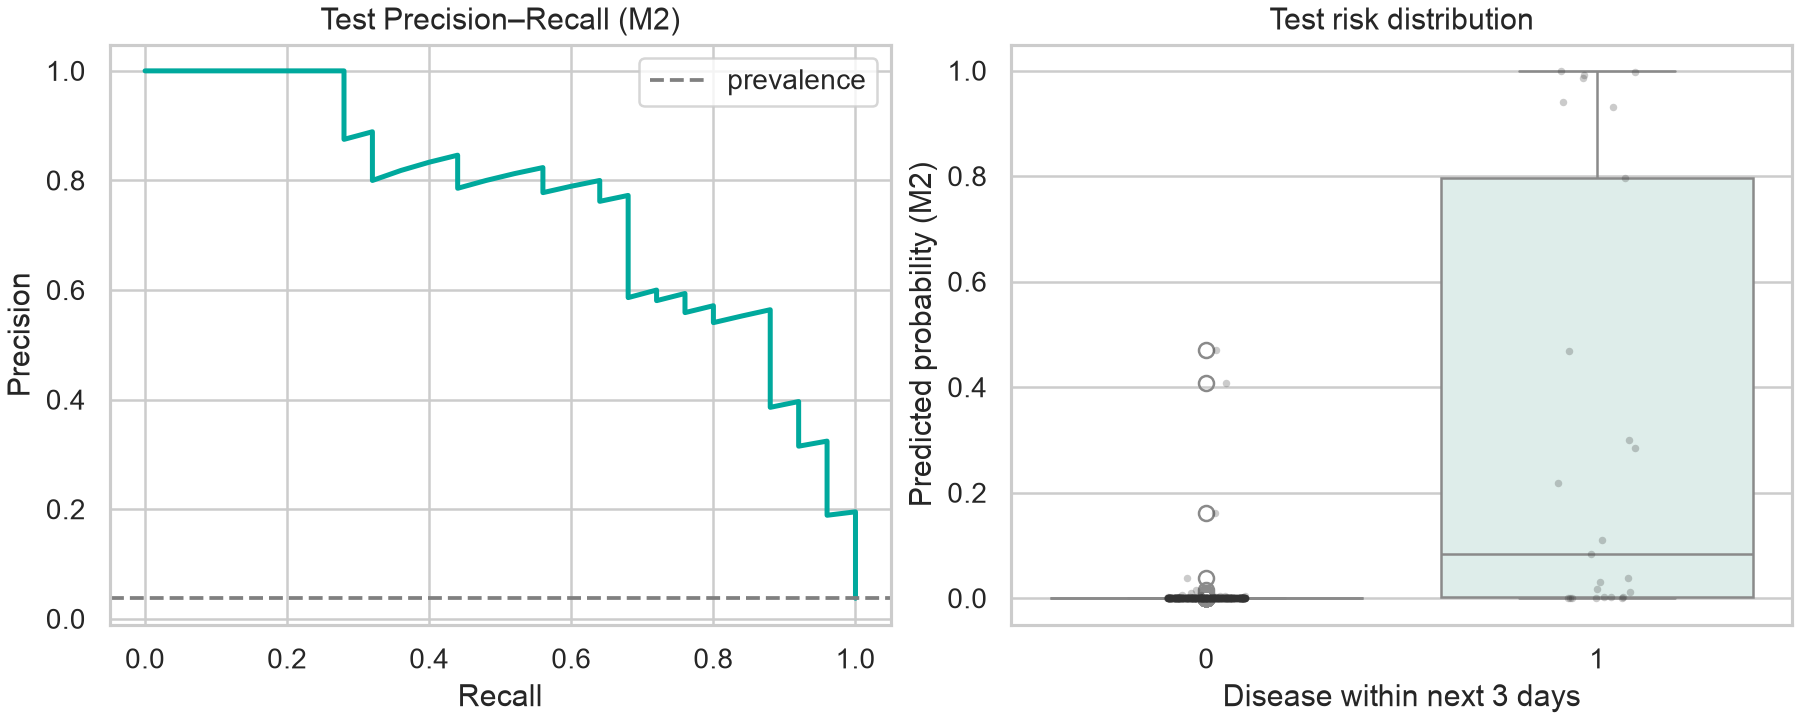
\includegraphics[width=0.92\textwidth]{thesis_model_evaluation.png}
\caption{M2의 test Precision--Recall 곡선(좌)과 예측확률 분포(우). 점선은 양성 유병률(prevalence)이다.}
\label{fig:pr}
\end{figure}

\section*{고\;찰}
동일 test에서 기초모형(M0)보다 당일 활력모형(M1)$\cdot$변화량 포함모형(M2)의 AUPRC가 높았다. 당일 행동$\cdot$활력지표와 최근 3일 개체 기준선 대비 변화량 추가가 구분력 향상에 기여한 것으로 해석되며, 사전 가설(H2)과 방향이 일치한다. 다만 본 결과는 관찰연관이며 인과를 주장하지 않는다.

한계는 명확하다. 자료는 실제 농장과 무관한 합성자료이며 외부 농장 검증이 없다. 수의사 확인 시점은 실제 임상발현보다 늦을 수 있고, 고온$\cdot$다습 및 카메라 사각지대는 질병성 활력 저하와 혼동될 수 있다. 돈방$\cdot$사양관리 차이는 지름길 학습의 원인이 될 수 있다. M0의 test 민감도 0은 임계값의 분할 간 일반화 실패를 보여 주며, 운영 임계값은 현장 목표 민감도와 허용 경보량을 기준으로 재설정해야 한다.

결론적으로, 본 합성자료 분석에서 최근 3일 활력 변화량을 포함한 모형이 기초모형보다 높은 AUPRC를 보였다. 모형 출력은 진단이 아니라 수의사 확인이 필요한 개체의 관찰 우선순위 보조정보로만 해석한다. 현장 적용 전에는 외부 검증, 라벨 정확성 검토, 비용--민감도 분석이 필요하다.

\vspace{0.6em}
\begin{center}\rule{0.92\textwidth}{0.4pt}\end{center}

\noindent\textbf{핵심어:} 돼지, 활력도, 조기경보, 영상행동, 예측모형\\
\textbf{Keywords:} pig, vitality, early warning, video-based behavior, prediction model

\vspace{0.7em}
\meta{\textbf{이해상충:} 없음.}
\meta{\textbf{연구비:} 해당 없음(교육용 분석).}
\meta{\textbf{자료 고지:} 본 초록의 수치$\cdot$개체$\cdot$이벤트가 실제 농장 또는 임상기록과 무관한 합성자료임을 명시한다.}
\meta{\textbf{AI 사용:} 초고 작성에 생성형 AI를 보조로 사용하였으며, 수치$\cdot$코드$\cdot$해석은 원자료 실행 결과와 대조하여 확인하였다. 최종 책임은 작성자에게 있다.}

\vspace{0.8em}
\begin{thebibliography}{9}
\bibitem{Matthews2016}
Matthews SG, Miller AL, Clapp J, Pl\"otz T, Kyriazakis I. Early detection of health and welfare compromises through automated detection of behavioural changes in pigs. \textit{Vet J}. 2016;217:43--51.
\bibitem{Fernandez2017}
Fern\'andez-Carri\'on E, Mart\'inez-Avil\'es M, L\'opez Garc\'ia-Baones A, et al. Motion-based video monitoring for early detection of livestock diseases: The case of African swine fever. \textit{PLoS One}. 2017;12(9):e0183793.
\end{thebibliography}

\end{document}
